% Provenance (never printed): old premiere S material on the oceanic lithosphere
% (ophiolite-type layering, peridotite and gabbro, partial melting by decompression
% at the ridge, hydrothermalism, cooling and subsidence of the lithosphere with
% age); see sources/book2/PROVENANCE.md. Melting from figdata/grade-11/
% ridge_melting.py (adiabat and Hirschmann solidus), depth against age from
% depth_age.py (ETOPO1 and the Seton 2020 age grid). Partial melting is re-founded
% in Year 2 (mantle-melting); fault is Book 1's (g7), normal fault is defined here.
\chapter{Ocean Ridges and the Oceanic Lithosphere}\label{ch:g11:ocean-ridges}

In February 1977 a camera sled towed 2500 metres down over the Galápagos
Rift, in the eastern Pacific, photographed the bare black lava of the ridge
frame after frame. Then its thermometer recorded a small rise in the
temperature of the water, and on the photographs the lava was covered with
hundreds of white clams. A few days later the submersible \emph{Alvin}
took two geologists down to the spot: warm, shimmering water was flowing out
of cracks in the lava, and around it lived clams as long as a forearm,
mussels and white crabs; on a later dive, tubeworms with red tops. Nobody had
expected life there, so no biologist was on board. This chapter explains
what the geologists had found: how the ocean floor is made at the ridges,
why it is hot there, and what becomes of it as it moves away.
% ledger: whoi:alvin-1977

\begin{recall}
At the ridges new ocean floor is made and moves away on both sides, so that
its age grows with distance from the axis; the ridges form a system about
\qty{65000}{km} long, with a rift valley along slow ridges and a smooth crest
along fast ones (\cref{ch:g11:drift-to-spreading}). Plates move apart across
a ridge at a few centimetres a year, faster across the East Pacific Rise than
across the Mid-Atlantic Ridge (\cref{ch:g11:plate-motions}). The \omterm{def:g11:lithosphere-asthenosphere:lithosphere}{lithosphere}
is the rigid outer shell, the \omterm{def:g11:lithosphere-asthenosphere:lithosphere}{asthenosphere} beneath it flows; the temperature
of the \omterm{def:g11:lithosphere-asthenosphere:lithosphere}{asthenosphere} rises by only about \qty{0.45}{\celsius} per kilometre
of depth, and the melting temperature of mantle rock rises with depth
(\cref{ch:g11:lithosphere-asthenosphere}). Magma is molten rock below the
surface, basalt the dark rock that lava makes when it cools, and a fault a
break along which rocks have moved (Book 1, grades 6 and 7).
\end{recall}
% ledger: noaa:ridge, katsura10:adiabat, hirschmann:solidus

\section{The oceanic lithosphere}

Two rocks that are rare at the surface of the continents make most of the
\omterm{def:g11:ocean-ridges:oceanic-lithosphere}{oceanic lithosphere}.

\begin{definition}[Peridotite]\label{def:g11:ocean-ridges:peridotite}
\emph{Peridotite}\index{peridotite} is a dark, coarse-grained rock made
mostly of the mineral olivine, with some pyroxene. It is usually green and
dense. Much of the Earth's mantle is believed to be made of peridotite.
\end{definition}

\begin{definition}[Gabbro]\label{def:g11:ocean-ridges:gabbro}
\emph{Gabbro}\index{gabbro} is a dark, coarse-grained igneous rock made
mainly of plagioclase feldspar and pyroxene. It has the same composition as
basalt, but it crystallised slowly, deep underground, which gave its crystals
time to grow. It is the most abundant rock of the deep \omterm{def:g11:ocean-ridges:oceanic-lithosphere}{oceanic crust}.
\end{definition}
% ledger: geo:peridotite, geo:gabbro

The minerals named here, olivine, pyroxene and feldspar, are described in
\cref{ch:g11:minerals}.

\begin{omfigure}
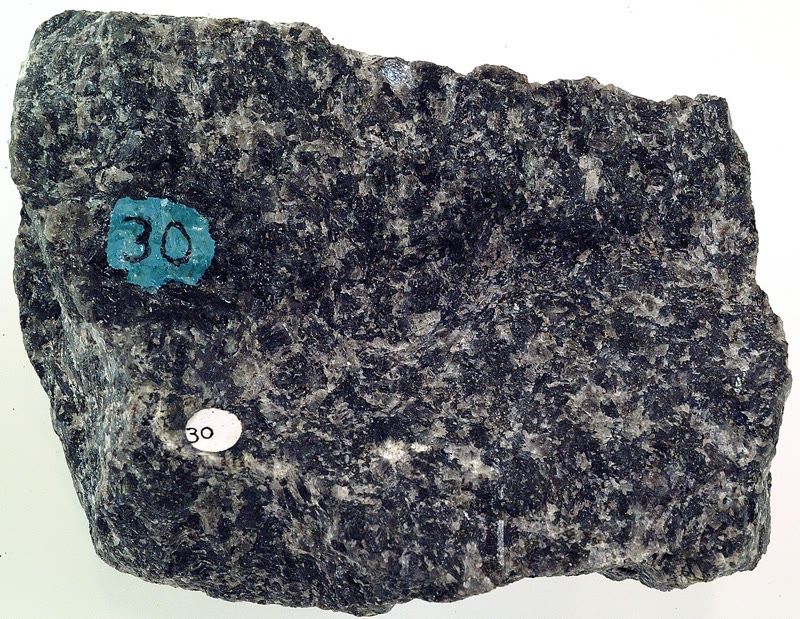
\includegraphics[height=4.2cm]{images/book2/g11-geodil-gabbro.jpg}\hspace{0.03\linewidth}%
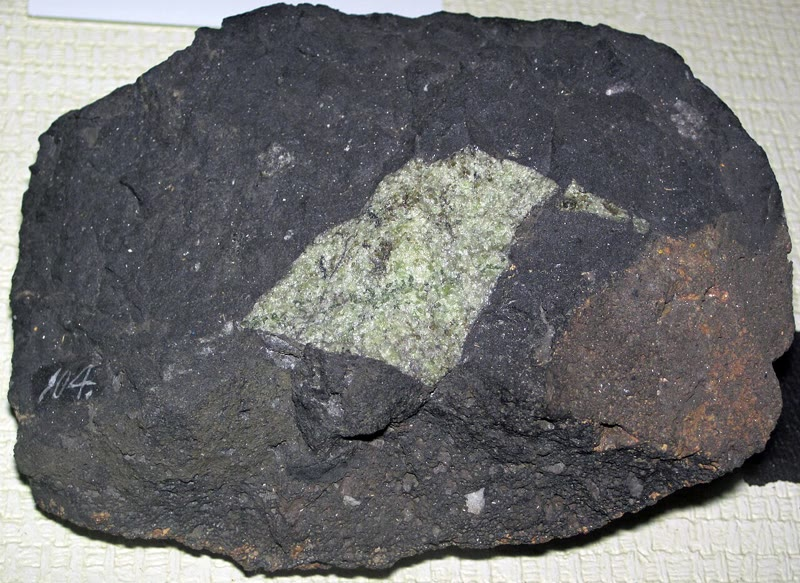
\includegraphics[height=4.2cm]{images/book2/g11-stjohn-peridotite.jpg}

{\small Left: \omterm{def:g11:ocean-ridges:gabbro}{gabbro}, \qty{9}{cm} across, with dark pyroxene and pale
feldspar crystals large enough to see; photograph Darla Sondrol (CC0).
Right: a lump of green \omterm{def:g11:ocean-ridges:peridotite}{peridotite} from the mantle, carried up inside the
black basalt lava of a volcano in Arizona; photograph James St.~John (CC~BY~2.0).}
\end{omfigure}
% ledger: photo:g11-gabbro, photo:g11-peridotite

\begin{definition}[Oceanic crust; oceanic lithosphere]\label{def:g11:ocean-ridges:oceanic-lithosphere}
The \emph{oceanic crust}\index{oceanic crust} is the crust of the ocean
floor: about \qty{7}{km} of basalt and \omterm{def:g11:ocean-ridges:gabbro}{gabbro}, made at the ridges. The
\emph{oceanic lithosphere}\index{oceanic lithosphere} is the oceanic crust
together with the rigid \omterm{def:g11:ocean-ridges:peridotite}{peridotite} of the uppermost mantle beneath it.
\end{definition}

Seismic surveys all over the oceans give the \omterm{def:g11:ocean-ridges:oceanic-lithosphere}{oceanic crust} an average
thickness of \qty{7.1}{km}, give or take \qty{0.8}{km}, away from fracture
zones and hotspots. Its layers are known from deep drilling and from slices
of old ocean floor pushed up onto the continents. In 2005 a drill ship
finished a hole \qty{1507}{m} deep into 15-million-year-old crust of the
eastern Pacific, the first to go from the lavas, through the dykes, into the
\omterm{def:g11:ocean-ridges:gabbro}{gabbros}:
% ledger: white92:crust, iodp1256:section, geo:peridotite

\begin{itemize}
  \item at the top, a thin cover of \emph{sediments}, absent at the ridge
        axis and thicker on older floor;
  \item more than \qty{800}{m} of \emph{basalt lavas}, erupted on the sea
        floor as sheets and as \emph{pillows}, rounded tubes and blobs of
        lava with a glassy skin;
  \item the \emph{sheeted dykes}, \qty{346}{m} in this hole: hundreds of
        vertical sheets of basalt, each the frozen crack through which magma
        rose to an eruption, side by side like the pages of a book;
  \item \emph{\omterm{def:g11:ocean-ridges:gabbro}{gabbro}}, reached \qty{1407}{m} below the sea floor, the magma
        that crystallised slowly below the dykes, down to the \omterm{def:g11:seismic-structure:moho}{Moho};
  \item below the \omterm{def:g11:seismic-structure:moho}{Moho}, the \emph{\omterm{def:g11:ocean-ridges:peridotite}{peridotite}} of the mantle.
\end{itemize}
% ledger: iodp1256:section, geo:basalt-ridges, geo:gabbro

\begin{omfigure}
\begin{tikzpicture}[x=1cm, y=-0.55cm, font=\footnotesize]
% to scale in depth: lavas 0.8 km, dykes 0.35 km (iodp1256:section), crust 7.1 km (white92:crust)
  \fill[omLithAlluv] (0,-0.25) rectangle (2.4,0);
  \fill[lith basalt] (0,0) rectangle (2.4,0.8);
  \fill[omLithBasalt!60] (0,0.8) rectangle (2.4,1.15);
  \foreach \x in {0.15,0.35,...,2.3} \draw[black!55, line width=0.3pt] (\x,0.8) -- (\x,1.15);
  \fill[lith gabbro] (0,1.15) rectangle (2.4,7.1);
  \fill[lith peridotite] (0,7.1) rectangle (2.4,9.0);
  \draw (0,-0.25) rectangle (2.4,9.0);
  \draw[line width=0.9pt] (0,7.1) -- (2.4,7.1);
  \foreach \d in {0,2,4,6,8} {\draw (-0.1,\d) -- (0,\d); \node[anchor=east] at (-0.1,\d) {\d};}
  \node[rotate=90, anchor=south] at (-0.75,4.5) {depth below the sea floor (\unit{km})};
  \draw[black!60] (2.4,-0.13) -- (2.7,-1.0) -- (2.85,-1.0);
  \node[anchor=west] at (2.85,-1.0) {sediments};
  \draw[black!60] (2.4,0.4) -- (2.7,0.25) -- (2.85,0.25);
  \node[anchor=west] at (2.85,0.25) {lavas: pillows and sheet flows};
  \draw[black!60] (2.4,0.98) -- (2.7,1.6) -- (2.85,1.6);
  \node[anchor=west] at (2.85,1.6) {sheeted dykes};
  \node[anchor=west] at (2.55,4.1) {gabbro};
  \node[anchor=west] at (2.55,7.1) {Moho};
  \node[anchor=west] at (2.55,8.05) {peridotite of the mantle};
  \draw[decorate, decoration={brace, amplitude=5pt}] (7.9,0) -- (7.9,7.1)
    node[midway, right=7pt, align=left] {oceanic crust\\about \qty{7}{km}};
\end{tikzpicture}

{\small The layers of the \omterm{def:g11:ocean-ridges:oceanic-lithosphere}{oceanic crust}, to scale in depth. The thicknesses of
the lavas and dykes are those of the deep hole drilled in the eastern Pacific;
the total thickness is the average from seismic surveys. The sediment cover
grows thicker with the age of the floor.}
\end{omfigure}
% ledger: iodp1256:section, white92:crust

\begin{omfigure}
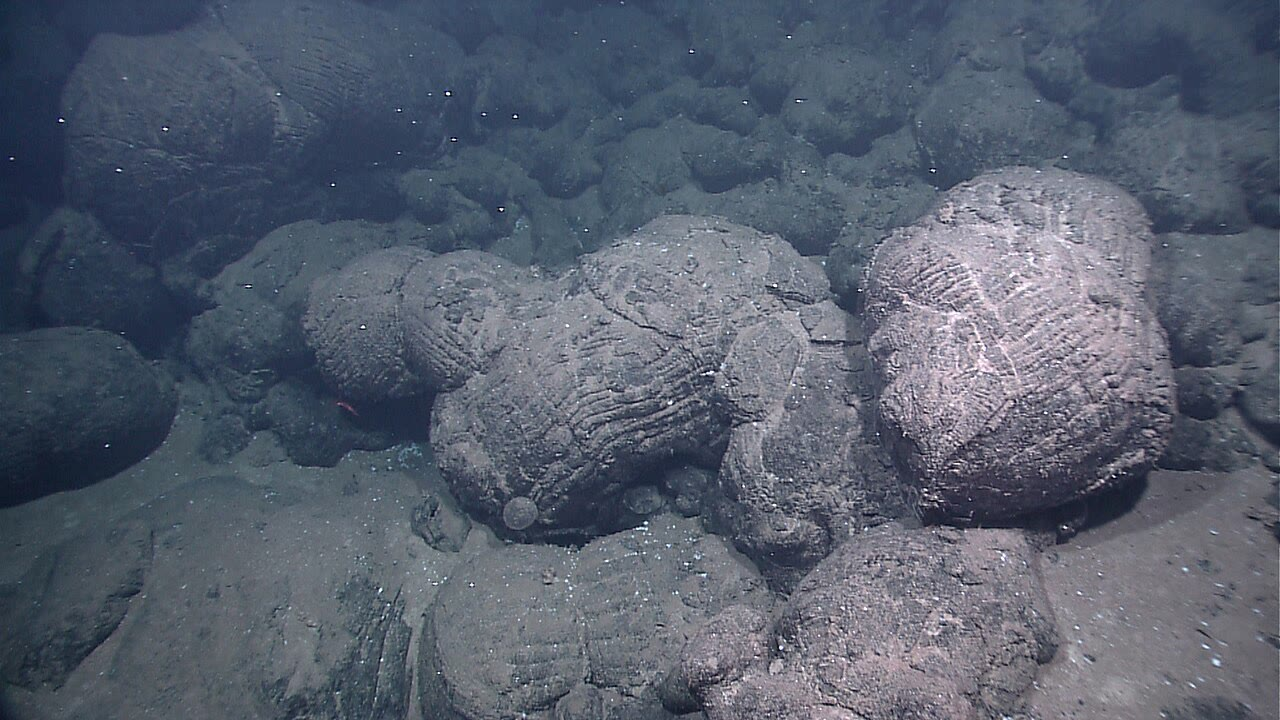
\includegraphics[width=0.8\linewidth]{images/book2/g11-noaa-pillow-lava.jpg}

{\small Pillow lava on the Galápagos Rift, about 2500 metres down,
photographed by a remotely operated vehicle in 2011. Each pillow is a tongue
of lava that froze from the outside the moment it met the cold sea water.
Photograph: NOAA Okeanos Explorer Program (public domain).}
\end{omfigure}
% ledger: photo:g11-pillow-lava, whoi:alvin-1977 (depth of the rift floor)

\section{Melting without heating}

The mantle beneath a ridge is solid \omterm{def:g11:ocean-ridges:peridotite}{peridotite}, as everywhere else. Yet
\qty{7}{km} of basalt and \omterm{def:g11:ocean-ridges:gabbro}{gabbro}, a molten rock frozen, come out of it. Where
does the melt come from?

\begin{definition}[Partial melting; decompression melting]\label{def:g11:ocean-ridges:partial-melting}
\emph{Partial melting}\index{partial melting} is the melting of only part
of a rock: some of its minerals, or some of their components, melt, while
the rest stays solid. \emph{Decompression melting}\index{decompression
melting} is the partial melting of a rock that rises, and so is less and
less squeezed, without being heated.
\end{definition}

As two plates move apart, the \omterm{def:g11:lithosphere-asthenosphere:lithosphere}{asthenosphere} rises beneath the ridge to fill
the gap. It rises too fast to lose much heat, so its temperature falls only
by about \qty{0.45}{\celsius} per kilometre on the way up. Its melting
temperature, which depends on the pressure, falls much faster: about
\qty{3.9}{\celsius} per kilometre at a depth of \qty{50}{km}. At some depth
the rising rock reaches its melting temperature and starts to melt, although
no heat has been added.
% ledger: katsura10:adiabat, hirschmann:solidus, white92:crust; computed in
% figdata/grade-11/ridge_melting.py (solidus_slope_50km 3.89)

\begin{method}[Where does the rising mantle melt?]\label{met:g11:ocean-ridges:melting}
\begin{enumerate}
  \item Write the temperature of the rising rock at each depth: its
        potential temperature (the temperature it would have at the surface)
        plus \qty{0.45}{\celsius} per kilometre of depth.
  \item Write the melting temperature of the rock at each depth, from the
        pressure at that depth.
  \item Find the depth where the two are equal. Deeper, the rock is solid;
        shallower, it is partly molten.
\end{enumerate}
\end{method}

\begin{omfigure}
\begin{tikzpicture}
\begin{axis}[omrecord, omdepth, width=0.72\linewidth, height=6.4cm, xmin=1100, xmax=1700, ymin=0, ymax=150,
  xlabel={temperature (\unit{\celsius})}, ylabel={depth (\unit{km})},
  xticklabel style={/pgf/number format/set thousands separator={}}, clip=true]
% computed in figdata/grade-11/ridge_melting.py; ledger: katsura10:adiabat, hirschmann:solidus, data:prem
\addplot[omProp, line width=1.0pt] table[x=solidus, y=z] {figdata/out/grade-11-ridge_melting-curves.dat};
\addplot[omDef, line width=1.0pt] table[x=ad1300, y=z] {figdata/out/grade-11-ridge_melting-curves.dat};
\addplot[omDef, densely dashed, line width=0.9pt] table[x=ad1400, y=z] {figdata/out/grade-11-ridge_melting-curves.dat};
\addplot[only marks, mark=*, mark size=1.8pt, black] coordinates {(1324.3,54.1) (1438.3,85.0)};
\node[font=\scriptsize, anchor=east, align=right] at (axis cs:1316,62) {melting begins,\\at \qty{54}{km}};
\node[font=\scriptsize, anchor=east] at (axis cs:1432,89) {\qty{85}{km}};
\node[font=\scriptsize, text=omProp, anchor=west, align=left] at (axis cs:1560,40) {melting\\temperature};
\node[font=\scriptsize, text=omDef, anchor=east, align=right] at (axis cs:1318,128) {rising mantle,\\$T_p = \qty{1300}{\celsius}$};
\node[font=\scriptsize, text=omDef, anchor=west, align=left] at (axis cs:1476,140) {$T_p = \qty{1400}{\celsius}$};
\end{axis}
\end{tikzpicture}

{\small The temperature of mantle rock rising beneath a ridge (blue) and its
melting temperature (orange), against depth. Rock with a potential
temperature of \qty{1300}{\celsius} starts to melt \qty{54}{km} down; rock
\qty{100}{\celsius} hotter (dashed) already at \qty{85}{km}. Melting
temperature of dry \omterm{def:g11:ocean-ridges:peridotite}{peridotite} from experiments (Hirschmann, 2000).}
\end{omfigure}
% values: onset_1300_km 54.1, onset_1400_km 85.0, t_onset_1300 1324 (ridge_melting.py)

\begin{example}[The depth of melting]\label{ex:g11:ocean-ridges:onset}
For a mantle of potential temperature \qty{1300}{\celsius}, the rising rock
is at $1300 + 0.45 \times 54 \approx \qty{1324}{\celsius}$ when it reaches
\qty{54}{km}, exactly its melting temperature at that depth: melting begins
about \qty{54}{km} down. Above that depth it goes on melting as it rises.
\end{example}

Only a small fraction of the \omterm{def:g11:ocean-ridges:peridotite}{peridotite} melts, and the melt is not \omterm{def:g11:ocean-ridges:peridotite}{peridotite}:
it is basalt. Basalt melts gather from the whole melting region, which reaches
from the onset depth up to the base of the crust; being lighter than the solid
rock around them, they rise to the ridge axis. There part of the magma erupts
as lava, part freezes in the cracks it rose through as dykes, and part
crystallises slowly below as \omterm{def:g11:ocean-ridges:gabbro}{gabbro}. The solid \omterm{def:g11:ocean-ridges:peridotite}{peridotite} left behind,
depleted of its basalt, becomes the mantle part of the \omterm{def:g11:ocean-ridges:oceanic-lithosphere}{oceanic lithosphere}.
% ledger: asimow01:morb, geo:basalt-ridges, white92:crust

Where a ridge crosses a region of hotter mantle, around a hotspot, melting
begins deeper, a longer column of rock melts and more basalt is made: there
the crust is about \qty{10}{km} thick instead of 7. Conversely, beneath very
slow ridges the rising mantle has time to lose heat, melts less, and makes an
unusually thin crust.
% ledger: white92:crust

\begin{omfigure}
\begin{tikzpicture}[font=\footnotesize]
  % schematic section across a ridge axis, not to scale
  \fill[omSea!45] (-6,0) rectangle (6,1.2);
  \fill[lith basalt] (-6,0) -- (-0.25,0) -- (-0.25,-0.35) -- (-6,-0.6) -- cycle;
  \fill[lith basalt] (6,0) -- (0.25,0) -- (0.25,-0.35) -- (6,-0.6) -- cycle;
  \fill[lith gabbro] (-6,-0.6) -- (-0.25,-0.35) -- (-0.25,-1.4) -- (-6,-1.6) -- cycle;
  \fill[lith gabbro] (6,-0.6) -- (0.25,-0.35) -- (0.25,-1.4) -- (6,-1.6) -- cycle;
  \fill[lith basalt] (-0.3,0) rectangle (0.3,-0.35);
  \fill[lith gabbro] (-0.3,-0.35) rectangle (0.3,-1.45);
  \fill[omProp!70] (-0.8,-0.75) .. controls (-0.4,-0.55) and (0.4,-0.55) .. (0.8,-0.75)
     .. controls (0.4,-0.95) and (-0.4,-0.95) .. (-0.8,-0.75);
  \fill[omProp!70] (-0.12,0) rectangle (0.12,-0.62);
  \fill[lith peridotite] (-6,-1.6) -- (-0.25,-1.4) -- (0.25,-1.4) -- (6,-1.6) -- (6,-5) -- (-6,-5) -- cycle;
  % melting region
  \fill[omProp!35] (-3.2,-1.5) -- (0,-4.0) -- (3.2,-1.5) -- cycle;
  \node[align=center] at (0,-2.95) {melting region};
  % isotherms deepening away from the axis
  \draw[omDef!70!black, densely dashed] (-6,-2.6) .. controls (-2.5,-2.0) and (-1,-1.1) .. (0,-1.0) .. controls (1,-1.1) and (2.5,-2.0) .. (6,-2.6);
  \draw[omDef!70!black, densely dashed] (-6,-4.2) .. controls (-3,-3.6) and (-1.2,-2.0) .. (0,-1.9) .. controls (1.2,-2.0) and (3,-3.6) .. (6,-4.2);
  \node[text=omDef!70!black, anchor=west] at (6.05,-2.6) {\qty{800}{\celsius}};
  \node[text=omDef!70!black, anchor=west] at (6.05,-4.2) {\qty{1200}{\celsius}};
  % flow arrows
  \draw[-{Stealth[length=5pt]}, line width=0.9pt] (0,-4.9) -- (0,-4.2);
  \draw[-{Stealth[length=5pt]}, line width=0.9pt] (-1.2,-4.8) .. controls (-1.0,-3.8) and (-2.2,-3.2) .. (-3.6,-3.2);
  \draw[-{Stealth[length=5pt]}, line width=0.9pt] (1.2,-4.8) .. controls (1.0,-3.8) and (2.2,-3.2) .. (3.6,-3.2);
  \draw[-{Stealth[length=5pt]}, line width=1.1pt] (-2,0.6) -- (-4,0.6);
  \draw[-{Stealth[length=5pt]}, line width=1.1pt] (2,0.6) -- (4,0.6);
  \node[anchor=south] at (-3,0.65) {plate};
  \node[anchor=south] at (3,0.65) {plate};
  \node[anchor=west] at (1.0,-0.8) {magma lens};
  \node[anchor=east] at (-6.05,-0.3) {lavas};
  \node[anchor=east] at (-6.05,-1.1) {gabbro};
  \node[anchor=east] at (-6.05,-3.3) {mantle};
  \node[anchor=north] at (0,-5.05) {the mantle rises and melts};
\end{tikzpicture}

{\small A section across a ridge axis (a drawing, not to scale). The mantle
rises beneath the axis and partly melts; the melt gathers in a magma lens
beneath the axis and builds the crust, which the plates carry away on both
sides. Lines of equal temperature (dashed) lie close to the surface at the
axis and deeper and deeper away from it: the \omterm{def:g11:lithosphere-asthenosphere:lithosphere}{lithosphere} thickens as it
cools.}
\end{omfigure}

\section{Fast and slow ridges}

Ridges open at very different speeds. Computed from the rotation poles of
\cref{ch:g11:plate-motions}, the East Pacific Rise at \ang{30} South opens at
\qty{14.6}{cm} a year, the Mid-Atlantic Ridge at the same latitude at
\qty{3.3}{cm} a year. The shape of the axis is not the same.
% ledger: nnr56:poles (computed in plate_velocities.py: epr30s_speed 145.8, atl30s_speed 32.7)

Along slow ridges, the axis is a valley 1 to \qty{2}{km} deep and 20 to
\qty{30}{km} wide. Too little magma reaches the axis to fill the gap
continuously: the cold, brittle \omterm{def:g11:lithosphere-asthenosphere:lithosphere}{lithosphere} is pulled apart and breaks along
faults.

\begin{definition}[Normal fault]\label{def:g11:ocean-ridges:normal-fault}
A \emph{normal fault}\index{normal fault} is an inclined fault along which
the block above the fault plane has moved down relative to the block below
it. Normal faults form where the crust is stretched.
\end{definition}

The valley of a slow ridge is a block that has dropped between \omterm{def:g11:ocean-ridges:normal-fault}{normal faults}
facing each other; nearly all of them dip toward the axis. Such a down-dropped
block between \omterm{def:g11:ocean-ridges:normal-fault}{normal faults} is called a \emph{graben}.
% ledger: buck05:valley, usgs:normal-fault

Along fast ridges, magma arrives often enough to fill the gap. The axis is a
smooth, gentle high, above a lens of magma that lies beneath it.
% ledger: buck05:valley, noaa:ridge

\begin{omfigure}
\begin{tikzpicture}[font=\footnotesize, x=0.24cm, y=0.9cm]
  % slow ridge: axial valley between normal faults (not to scale, vertical exaggeration)
  \begin{scope}
    \fill[omSea!45] (-15,-0.7) rectangle (15,1.6);
    \fill[lith basalt] (-15,0.9) -- (-9,0.9) -- (-8.5,0.2) -- (-6,0.2) -- (-5.5,-0.6) -- (5.5,-0.6)
      -- (6,0.2) -- (8.5,0.2) -- (9,0.9) -- (15,0.9) -- (15,-2.2) -- (-15,-2.2) -- cycle;
    \draw[black!70] (-15,0.9) -- (-9,0.9) -- (-8.5,0.2) -- (-6,0.2) -- (-5.5,-0.6) -- (5.5,-0.6)
      -- (6,0.2) -- (8.5,0.2) -- (9,0.9) -- (15,0.9);
    \draw[fault] (-9,0.9) -- (-7.4,-2.2);
    \draw[fault] (-6,0.2) -- (-4.6,-2.2);
    \draw[fault] (9,0.9) -- (7.4,-2.2);
    \draw[fault] (6,0.2) -- (4.6,-2.2);
    % slip arrows on the hanging walls (the axis side of each fault): down along the fault
    \foreach \x/\y/\s in {-7.9/-0.5/1, -5.0/-1.3/1, 7.9/-0.5/-1, 5.0/-1.3/-1} {
      \draw[-{Stealth[length=3pt]}, omProp, line width=0.8pt] (\x+0.9*\s,\y+0.45) -- ++(0.3*\s,-0.6);
    }
    \draw[-{Stealth[length=5pt]}, line width=1pt] (-11,1.25) -- (-14,1.25);
    \draw[-{Stealth[length=5pt]}, line width=1pt] (11,1.25) -- (14,1.25);
    \node at (0,-0.25) {axial valley};
    \node[anchor=north, align=center] at (0,-2.25) {slow ridge: a valley\\between normal faults};
  \end{scope}
  % fast ridge
  \begin{scope}[xshift=8.2cm]
    \fill[omSea!45] (-15,0) rectangle (15,1.6);
    \fill[lith basalt] (-15,0.3) .. controls (-6,0.4) and (-2,0.9) .. (0,0.95) .. controls (2,0.9) and (6,0.4) .. (15,0.3)
      -- (15,-2.2) -- (-15,-2.2) -- cycle;
    \fill[omProp!75] (-2.5,-0.9) .. controls (-1,-0.7) and (1,-0.7) .. (2.5,-0.9) .. controls (1,-1.1) and (-1,-1.1) .. (-2.5,-0.9);
    \draw[black!70] (-15,0.3) .. controls (-6,0.4) and (-2,0.9) .. (0,0.95) .. controls (2,0.9) and (6,0.4) .. (15,0.3);
    \node[anchor=north] at (0,-1.25) {magma lens};
    \draw[-{Stealth[length=5pt]}, line width=1pt] (-8,1.25) -- (-14,1.25);
    \draw[-{Stealth[length=5pt]}, line width=1pt] (8,1.25) -- (14,1.25);
    \node at (0,1.3) {axial high};
    \node[anchor=north, align=center] at (0,-2.25) {fast ridge: a gentle high\\over a magma lens};
  \end{scope}
\end{tikzpicture}

{\small Sections across a slow and a fast ridge (drawings, not to scale; the
height is exaggerated). Left: the axial valley of a slow ridge, 1 to
\qty{2}{km} deep, has dropped between \omterm{def:g11:ocean-ridges:normal-fault}{normal faults} dipping toward the axis
(orange arrows: the blocks above the faults slide down). Right: a fast ridge
rises gently above a lens of magma.}
\end{omfigure}
% ledger: buck05:valley

\begin{example}[A slow and a fast ridge]\label{ex:g11:ocean-ridges:rates}
In a million years the East Pacific Rise at \ang{30} South makes
$\qty{14.6}{cm/yr} \times 10^6\ \text{years} = \qty{146}{km}$ of new ocean
floor, \qty{73}{km} on each side; the Mid-Atlantic Ridge at the same latitude
makes \qty{33}{km}, \qty{16.5}{km} on each side. The deep hole of the eastern
Pacific went into crust made at more than \qty{20}{cm} a year, among the
fastest spreading ever recorded.
\end{example}
% ledger: nnr56:poles (computed), iodp1256:section

\section{Hydrothermal vents}

The young crust at the axis is hot, and it is broken by cracks. Sea water
finds its way in.

\begin{definition}[Hydrothermal circulation; black smoker]\label{def:g11:ocean-ridges:hydrothermal}
\emph{Hydrothermal circulation}\index{hydrothermal circulation} is the flow
of sea water down through the cracks of the hot \omterm{def:g11:ocean-ridges:oceanic-lithosphere}{oceanic crust}, where it is
heated by the magma below and reacts with the rock, and back up to the sea
floor, where it comes out at \emph{hydrothermal vents}. A \emph{black
smoker}\index{black smoker} is a vent from which very hot water carrying
dissolved metals pours out; as it meets the cold sea water, iron sulfides and
other minerals precipitate as a black cloud, and build a chimney around the
vent.
\end{definition}
% ledger: whoi:vents

Black-smoker water typically leaves its chimney at about
\qty{350}{\celsius}, and vent waters can reach \qty{400}{\celsius}. They do not
boil, because two and a half kilometres of water press on them. The
chimneys can grow more than \qty{10}{m} high. Around the vents, bacteria draw
their energy from the hydrogen sulfide of the vent water, and feed tubeworms,
shrimp and mussels: the clams of the Galápagos Rift lived on this. Most
vents lie along the mid-ocean ridges.
% ledger: whoi:vents, whoi:alvin-1977

\begin{omfigure}
\begin{minipage}[c]{0.6\linewidth}\centering
\begin{tikzpicture}[font=\scriptsize, x=0.8cm, y=0.62cm]
  \fill[omSea!45] (0,0) rectangle (10,3);
  \fill[lith basalt] (0,0) rectangle (10,-4);
  \fill[omProp!70] (2,-4.6) .. controls (4,-4.0) and (6,-4.0) .. (8,-4.6) -- (8,-5) -- (2,-5) -- cycle;
  \node at (5,-4.7) {magma};
  \fill[black!75] (4.7,0) -- (4.85,1.6) -- (5.15,1.6) -- (5.3,0) -- cycle;
  \fill[black!45, opacity=0.8] (5,1.7) circle (0.35) (5.2,2.2) circle (0.45) (4.9,2.7) circle (0.4);
  \draw[-{Stealth[length=4pt]}, omDef, line width=0.9pt] (1,0) .. controls (1,-2.5) and (2.5,-3.6) .. (4.2,-3.5);
  \draw[-{Stealth[length=4pt]}, omDef, line width=0.9pt] (9,0) .. controls (9,-2.5) and (7.5,-3.6) .. (5.8,-3.5);
  \draw[-{Stealth[length=4pt]}, omProp, line width=1.1pt] (5,-3.3) -- (5,-0.1);
  \node[align=center, text=omDef!80!black] at (1.6,1.0) {cold sea\\water in};
  \node[align=left, anchor=west] at (5.6,1.4) {black smoker,\\about \qty{350}{\celsius}};
  \node[align=left, anchor=west, text=omProp!80!black, fill=white, fill opacity=0.85, text opacity=1, inner sep=1.5pt] at (5.3,-1.8) {heated,\\rises};
\end{tikzpicture}
\end{minipage}\hfill
\begin{minipage}[c]{0.3\linewidth}\centering
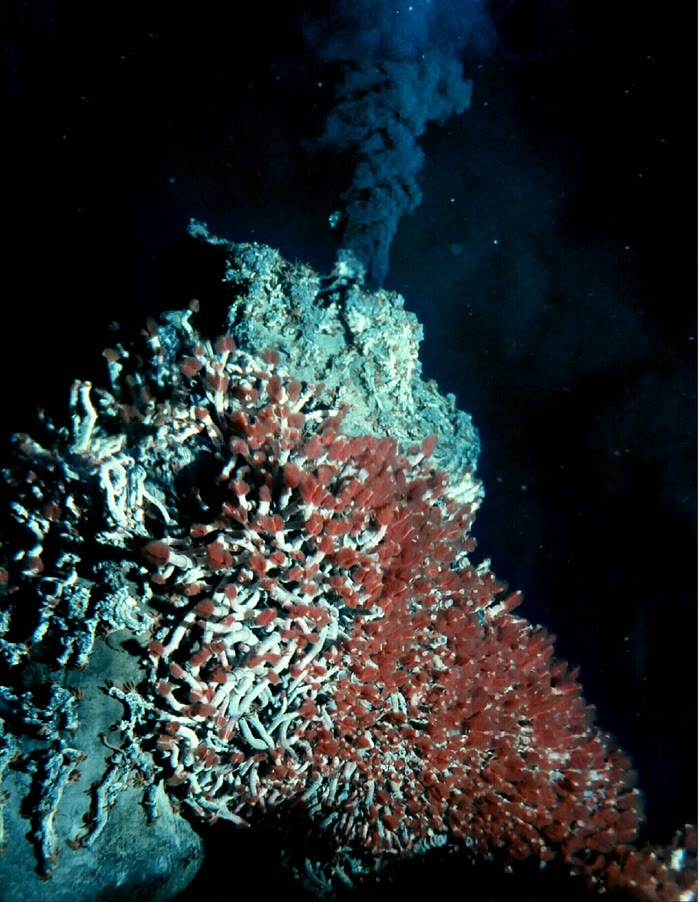
\includegraphics[width=\linewidth]{images/book2/g11-noaa-black-smoker.jpg}
\end{minipage}

{\small Left: \omterm{def:g11:ocean-ridges:hydrothermal}{hydrothermal circulation} at a ridge axis (a drawing, not to
scale). Right: a \omterm{def:g11:ocean-ridges:hydrothermal}{black smoker} on the Juan de Fuca Ridge, its chimney covered
with red-gilled tubeworms; photograph University of Washington and NOAA
(public domain).}
\end{omfigure}
% ledger: whoi:vents, photo:g11-black-smoker

\begin{history}[\emph{Alvin} on the Galápagos Rift, 1977]
The expedition, funded by the National Science Foundation, began on
8~February 1977 aboard the research ship \emph{Knorr}. The camera sled ANGUS,
towed \qty{2500}{m} down over the rift, recorded a rise in the temperature of
the water, and in the same frames its photographs showed hundreds of white
clams and brown mussel shells on the lava. On \emph{Alvin}'s dive 713, the
geologists Jack Corliss and Tjeerd van Andel found water at \qty{8}{\celsius}
shimmering out of the cracks, then up to \qty{17}{\celsius}, while the deep
water around was at \qty{2}{\celsius}; white clams up to \qty{30}{cm} long
covered an area about \qty{50}{m} across. No biologist was aboard: the
expedition had come for the hot water, and found a community of animals that
nobody had imagined.
\end{history}
% ledger: whoi:alvin-1977

\section{Cooling, thickening, sinking}

As it moves away from the axis, the \omterm{def:g11:lithosphere-asthenosphere:lithosphere}{lithosphere} cools from the top, through
the cold ocean above it. The cooled layer grows thicker with time: the
\omterm{def:g11:lithosphere-asthenosphere:lithosphere}{lithosphere} thickens, from a few kilometres at the axis to about a hundred
kilometres on old floor. Cooled rock contracts and becomes denser, so the
\omterm{def:g11:lithosphere-asthenosphere:lithosphere}{lithosphere} floats lower on the \omterm{def:g11:lithosphere-asthenosphere:lithosphere}{asthenosphere} (\omterm{def:g11:lithosphere-asthenosphere:isostasy}{isostasy},
\cref{ch:g11:lithosphere-asthenosphere}): the ocean floor sinks as it ages.
For a body that cools by conduction from its surface, the thickness of the
cooled layer grows like the square root of the time.
% ledger: ps77:depth-age, rs09:lab

\begin{proposition}[Depth of the ocean floor against its age]\label{prop:g11:ocean-ridges:depth-age}
On average, ocean floor of age $t$ (in millions of years) lies at the depth
\[
  d(t) = 2500 + 350\sqrt{t} \quad \text{metres} \qquad (0 \le t \le 70),
\]
and, for floor older than about 20 million years,
\[
  d(t) = 6400 - 3200\,e^{-t/62.8} \quad \text{metres}:
\]
the floor sinks quickly while it is young, then more and more slowly, toward
about \qty{6400}{m}. (Admitted: the formulas were fitted to the depths of the
North Pacific and North Atlantic, corrected for the weight of their
sediments, by Parsons and Sclater in 1977.)
\end{proposition}
% ledger: ps77:depth-age

The square root makes the young floor sink fast: in its first million years
the floor sinks by \qty{350}{m}, in the next three million years by another
\qty{350}{m}, and between 16 and 64 million years by \qty{1400}{m}, as much as
in its first sixteen million years. The exponential law describes how old
floor stops sinking: it behaves as if the cooling plate had a fixed thickness,
about \qty{125}{km}.
% ledger: ps77:depth-age

\begin{omfigure}
\begin{tikzpicture}
\begin{axis}[omrecord, omdepth, width=0.82\linewidth, height=6.2cm, xmin=0, xmax=180, ymin=2000, ymax=6600,
  xlabel={age of the ocean floor (millions of years)}, ylabel={depth (\unit{m})},
  yticklabel style={/pgf/number format/set thousands separator={}},
  legend style={font=\scriptsize, at={(0.5,-0.32)}, anchor=north, legend columns=3, /tikz/every even column/.append style={column sep=6pt}}, legend cell align=left]
% computed in figdata/grade-11/depth_age.py; ledger: data:etopo1, data:b2-seafloor-age, ps77:depth-age
\addplot[only marks, mark=*, mark size=1.3pt, black!70, error bars/.cd, y dir=both, y explicit]
  table[x=age, y=depth, y error minus=em, y error plus=ep] {figdata/out/grade-11-depth_age-bins.dat};
\addplot[omProp, line width=1.0pt] table[x=age, y=depth] {figdata/out/grade-11-depth_age-sqrt.dat};
\addplot[omDef, line width=1.0pt, densely dashed] table[x=age, y=depth] {figdata/out/grade-11-depth_age-exp.dat};
\legend{{measured: median and middle half}, {$2500 + 350\sqrt{t}$}, {$6400 - 3200\,e^{-t/62.8}$}}
\end{axis}
\end{tikzpicture}

{\small Depth of the ocean floor against its age: for each 5-million-year age
band, the median depth of all the one-degree cells of the world's oceans,
and the range of the middle half of them. Young floor follows the
square-root law closely; older floor lies shallower than the laws, because
its cells include sediments and volcanoes. Data: ETOPO1 (NOAA) and the
ocean-floor ages of Seton and others (2020); laws of Parsons and Sclater
(1977).}
\end{omfigure}
% values (depth_age.py): median 2.5-5 Myr 3114 (law 3178), 60-65 Myr 4648 (law 5267), fit a 2727 b 255

The measured depths of young floor agree with the law to within about
\qty{100}{m}. On older floor the measured medians lie several hundred metres
above the laws. The laws describe the depth of the floor itself, as if its
sediments were removed; the measured cells still carry their sediments,
which grow thicker with the age of the floor and are more than a kilometre
thick on the oldest floor of the western North Atlantic, and they include
seamounts and volcanic plateaus.
% ledger: ps77:depth-age; values from depth_age.py

Old \omterm{def:g11:ocean-ridges:oceanic-lithosphere}{oceanic lithosphere} is therefore thick, cold and dense. The next chapter
shows that it can become denser than the \omterm{def:g11:lithosphere-asthenosphere:lithosphere}{asthenosphere} beneath it, and sink
back into the mantle (\cref{ch:g11:subduction-zones}).

\section{Exercises}

\begin{exercise}[$\star$]\label{exo:g11:ocean-ridges:1}
Define \omterm{def:g11:ocean-ridges:peridotite}{peridotite} and \omterm{def:g11:ocean-ridges:gabbro}{gabbro}. Which of the two belongs to the \omterm{def:g11:ocean-ridges:oceanic-lithosphere}{oceanic crust},
and which to the mantle? \omterm{def:g11:ocean-ridges:gabbro}{Gabbro} has the same composition as basalt: why are
its crystals so much larger?
\end{exercise}

\begin{exercise}[$\star$]\label{exo:g11:ocean-ridges:2}
List the layers of the \omterm{def:g11:ocean-ridges:oceanic-lithosphere}{oceanic lithosphere} from the sea floor down. The deep
hole of the eastern Pacific reached \qty{1507}{m} below the sea floor: what
fraction of a \qty{7.1}{km} crust did it cross?
\end{exercise}

\begin{exercise}[$\star$]\label{exo:g11:ocean-ridges:3}
Using $d = 2500 + 350\sqrt{t}$, find the depth of ocean floor 0, 9 and 25
million years old.
\end{exercise}

\begin{exercise}[$\star$]\label{exo:g11:ocean-ridges:4}
Define a \omterm{def:g11:ocean-ridges:normal-fault}{normal fault}. At a slow ridge, what force makes \omterm{def:g11:ocean-ridges:normal-fault}{normal faults}, and
in which direction do the blocks above the faults move?
\end{exercise}

\begin{exercise}[$\star$]\label{exo:g11:ocean-ridges:5}
Black-smoker water comes out at about \qty{350}{\celsius}. Why does it not
boil? What is the black ``smoke''?
\end{exercise}

\begin{exercise}[$\star\star$]\label{exo:g11:ocean-ridges:6}
Using the melting figure: (1) at what depth does a mantle of potential
temperature \qty{1300}{\celsius} begin to melt, and at what temperature? (2)
And a mantle \qty{100}{\celsius} hotter? (3) Which of the two makes the
thicker crust? Why?
\end{exercise}

\begin{exercise}[$\star\star$]\label{exo:g11:ocean-ridges:7}
Rising mantle rock of potential temperature \qty{1300}{\celsius} is at
\qty{1345}{\celsius} at a depth of \qty{100}{km}, where its melting
temperature is \qty{1489}{\celsius}. (1) How far below its melting
temperature is it? (2) It starts to melt at \qty{54}{km}. By how many degrees
per kilometre, on average, has the gap closed on the way up? (3) Has the rock
been heated?
\end{exercise}

\begin{exercise}[$\star\star$]\label{exo:g11:ocean-ridges:8}
The East Pacific Rise opens at \qty{14.6}{cm} a year at \ang{30} South, the
Mid-Atlantic Ridge at \qty{3.3}{cm} a year. Assuming symmetric spreading, how
long does each ridge take to make \qty{1000}{km} of floor on one side?
\end{exercise}

\begin{exercise}[$\star\star$]\label{exo:g11:ocean-ridges:9}
The ridges are about \qty{65000}{km} long. Suppose they open on average at
\qty{5}{cm} a year and make a crust \qty{7.1}{km} thick. (1) What area of new
ocean floor do they make each year? (2) What volume of crust? (3) How long
would they take to make an area equal to that of the oceans,
\qty{3.6e8}{km^2}?
\end{exercise}

\begin{exercise}[$\star\star$]\label{exo:g11:ocean-ridges:10}
An axial valley is \qty{1.5}{km} deep. It dropped along two \omterm{def:g11:ocean-ridges:normal-fault}{normal faults}
facing each other, each dipping at \ang{60}. (1) By how much did each fault
move along its plane? (2) How far apart did the two sides move horizontally
because of the two faults? (3) The valley is \qty{25}{km} wide: did faulting
alone make it?
\end{exercise}

\begin{exercise}[$\star\star$]\label{exo:g11:ocean-ridges:11}
Using $d = 6400 - 3200\,e^{-t/62.8}$, find the depth of floor 25 and 100
million years old, and how much the floor sinks between these ages. Compare
the first value with that of the square-root law.
\end{exercise}

\begin{exercise}[$\star\star\star$]\label{exo:g11:ocean-ridges:12}
A column of mantle \qty{100}{km} thick cools by \qty{700}{\celsius} on
average. Rock contracts by $\alpha = 3.2 \times 10^{-5}$ of its length for
each degree of cooling. (1) By how much does the column shorten? (2) As it
sinks, sea water (\qty{1025}{kg/m^3}) fills the space above it; with a mantle
density of \qty{3380}{kg/m^3}, \omterm{def:g11:lithosphere-asthenosphere:isostasy}{isostasy} makes the floor sink by
$s = \rho_m\,\alpha\,\Delta T\,L/(\rho_m - \rho_w)$. Compute $s$. (3) Compare
with the total sinking that the exponential law allows, from \qty{2500}{m} to
\qty{6400}{m}.
\end{exercise}

\begin{exercise}[$\star\star\star$]\label{exo:g11:ocean-ridges:13}
Melting begins \qty{54}{km} down in a mantle at \qty{1300}{\celsius},
\qty{85}{km} down in one at \qty{1400}{\celsius}; in both, melting goes on up
to the base of the crust, about \qty{7}{km} down. (1) Compare the lengths of
the two melting columns. (2) If each kilometre of rising rock gave the same
amount of melt, how thick would the crust be over the hotter mantle, for a
\qty{7.1}{km} crust over the normal one? (3) Compare with the \qty{10.3}{km}
measured where ridges meet hotter mantle.
\end{exercise}

\begin{exercise}[$\star\star\star$]\label{exo:g11:ocean-ridges:14}
The measured median depths of the ocean floor are \qty{3114}{m} at an age of
\num{3.75} million years, \qty{4018}{m} at \num{22.5}, \qty{4465}{m} at
\num{42.5} and \qty{4648}{m} at \num{62.5}. (1) Compute the depth given by the
square-root law at each age, and the difference with the measurement. (2)
How does the difference change with age? (3) Explain it.
\end{exercise}

\begin{exercise}[$\star\star\star$]\label{exo:g11:ocean-ridges:15}
Water's critical point is at \qty{374}{\celsius} and \qty{22.064}{MPa}: above
that pressure, water does not boil at any temperature. (1) Compute the
pressure of the water \qty{2500}{m} down (sea water \qty{1025}{kg/m^3},
$g = \qty{9.8}{m/s^2}$, plus the atmosphere's \qty{0.1}{MPa}). (2) Can the
water of a vent boil at that depth, however hot it is? (3) Below about what
depth is this true for every vent?
\end{exercise}

\section{Problem: The Life of a Piece of Pacific Floor}

\begin{problem}[{Weekend problem --- from the ridge to the deep ocean}]
\label{pb:g11:ocean-ridges:1}
% values: EPR 30 S full rate 145.8 mm/yr (plate_velocities.py, nnr56:poles); depth law
% ps77:depth-age; crust white92:crust; alpha ps77; densities data:prem; median 60-65 Myr
% 4648 m (depth_age.py)
A piece of ocean floor is born today on the East Pacific Rise at \ang{30}
South, where the Pacific and Nazca plates move apart at \qty{14.6}{cm} a year.
It moves west with the Pacific plate. Take the spreading as symmetric, the
crust \qty{7.1}{km} thick, and the depth law $d = 2500 + 350\sqrt{t}$ metres
($t$ in millions of years).

\medskip
\noindent\textbf{Part I --- Birth at the ridge.}
\begin{enumerate}
  \item What is the half \omterm{def:g11:drift-to-spreading:spreading-rate}{spreading rate}, in centimetres a year and in
        kilometres per million years?
  \item At what depth is the piece of floor born?
  \item List the rocks it is made of, from the sea floor down to the base of
        the \omterm{def:g11:lithosphere-asthenosphere:lithosphere}{lithosphere}.
  \item The magma that made it came from the mantle below. Explain how the
        mantle melted without being heated.
  \item What volume of crust does this ridge make each million years, on
        both sides, for each kilometre of its length?
\end{enumerate}

\medskip
\noindent\textbf{Part II --- The journey.}
\begin{enumerate}[resume]
  \item How far from the ridge will the piece be after 1, 4, 16 and 64
        million years, if the rate stays the same?
  \item How long will it take to travel \qty{2000}{km}?
  \item Why may the real distance after 64 million years differ from the
        answer of question~6?
  \item Near the ridge, sea water circulates through the young crust and
        comes out at vents. Why does this circulation stop on old floor?
  \item On which plate does the piece travel, and toward which kind of
        plate boundary does that plate carry it, on its western side?
\end{enumerate}

\medskip
\noindent\textbf{Part III --- Sinking as it ages.}
\begin{enumerate}[resume]
  \item Compute its depth at 1, 4, 16 and 64 million years.
  \item By how much does it sink during its first 16 million years, and
        between 16 and 64 million years? Comment.
  \item At what age does it reach a depth of \qty{4000}{m}?
  \item Compare its depth at 64 million years with the exponential law,
        $6400 - 3200\,e^{-t/62.8}$.
  \item The measured median depth of ocean floor 60 to 65 million years old
        is \qty{4648}{m}. Explain the difference.
\end{enumerate}

\medskip
\noindent\textbf{Part IV --- Its density and its fate.}
\begin{enumerate}[resume]
  \item By 64 million years, take its \omterm{def:g11:lithosphere-asthenosphere:lithosphere}{lithosphere} as \qty{100}{km} thick and
        on average \qty{700}{\celsius} colder than the \omterm{def:g11:lithosphere-asthenosphere:lithosphere}{asthenosphere}. With
        $\alpha = 3.2 \times 10^{-5}$ per degree, by what fraction has the
        mantle part become denser? Starting from \qty{3380}{kg/m^3}, what is
        its density?
  \item Its crust is \qty{7.1}{km} thick, with a density of
        \qty{2900}{kg/m^3}. Compute the mean density of the whole
        \qty{100}{km} of \omterm{def:g11:lithosphere-asthenosphere:lithosphere}{lithosphere}.
  \item Compare with the \omterm{def:g11:lithosphere-asthenosphere:lithosphere}{asthenosphere} beneath it, taken at
        \qty{3380}{kg/m^3}.
  \item What can such a \omterm{def:g11:lithosphere-asthenosphere:lithosphere}{lithosphere} do when it reaches a trench?
  \item Conclude: at what depth does this piece of floor lie when it is 64
        million years old?
\end{enumerate}
\end{problem}
